\section{Turning Scores into Geometry}
\label{eg:geometry}

\paragraph{Sequential design.}
We generate feasible candidates, scout with inexpensive walks, and rescore a
shortlist with fresh samples. A selected cavity is inserted, the current
domain is updated, and the process repeats. Existing interfaces can then
be refined using Differential WoS. Independent rescoring reduces selection
noise, but selecting among several fresh estimates still requires simultaneous
coverage or another final check to support a certificate. Our ranking and
refinement studies evaluate a practical heuristic; they are separate from the
guarded validation experiment below.

\begin{figure}[t]
 \centering
 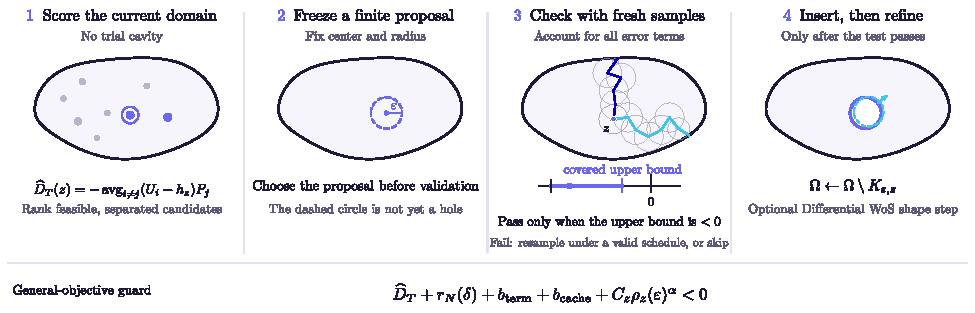
\includegraphics[width=\textwidth]{figures/pipeline.pdf}
 \caption{\textbf{From an insertion score to a finite geometric decision.} Score the current domain, freeze a center and radius, and validate with fresh samples before creating the cavity. The general-objective guard combines statistical uncertainty, oracle bias, and a finite-radius remainder bound. Its covered upper bound must be negative. A failed check leads to a valid resampling schedule or no insertion. The dashed cyan boundary shows optional subsequent shape refinement. This conditional certifying policy requires usable error bounds; the practical ranking studies and the cooling-specific finite-benefit test have separate scopes.}
 \label{fig:insertionpolicy}\label{fig:pipeline}
\end{figure}

\paragraph{General-objective acceptance.}
Suppose a known bound satisfies
\[
 |\J(\Omega_{\eps,z})-\J(\Omega)-\rho_z(\eps)\DT(z)|
 \le C_z\rho_z(\eps)^{1+\alpha}.
\]
At a preselected site, a valid statistical radius $r_N(\delta)$ and bias budget
$b=b_{\rm term}+b_{\rm cache}$ give the sufficient test
\begin{equation}
 \widehat{\DT}_N+r_N(\delta)+b+C_z\rho_z(\eps)^\alpha<0.
 \label{eg:eq:accept}
\end{equation}
The probability of accepting a non-improving insertion is then at most
$\delta$ (\cref{thm:certificate}). \Cref{fig:insertionpolicy} shows this conditional policy. A radius chosen after validation is covered
by the same event when the deterministic bound holds uniformly over allowed
radii. Existence of an asymptotic constant is insufficient: the test needs a
numerical upper bound. Across adaptive rounds, allocating summable conditional
failure probabilities controls the familywise error
(\cref{prop:freshvalidation}). Repeatedly inspecting a fixed-sample interval
without such a schedule is not covered.

\paragraph{A direct finite-benefit route for cooling.}
For $-\Delta u=f$ with bounded $0\le f\le F$ with zero Dirichlet walls in a bounded Lipschitz
three-dimensional domain $D$, let $J(D)=\int_Dfu$. A contained sphere
$\overline B_r(z)\Subset D$ has benefit
\begin{equation}
 J(D)-J(D\setminus\overline B_r(z))
 \ge 4\pi r\,(L_u-I_r^+)_+^2,
 \label{eg:eq:finitebenefit}
\end{equation}
on an event where $L_u\le u(z)$, provided
\[
I_r^+\ge\int_{B_r(z)}G_{B_r(z)}(z,y)f(y)\,dy.
\]
One may use $I_r^+=f_+r^2/6$ for a valid local upper source bound.
The difference-energy identity and the ball equilibrium potential bound the
benefit by the squared average cavity trace; the center Green identity
recovers that trace (\cref{thm:averagecertificate}). A clipped,
zero-terminal nonnegative-source WoS estimate enables a one-sided lower
confidence bound. The complete proof, sample range, and geometric guards are
in \cref{app:applicationcertificate}. The guarantee remains conditional on
the stated sampling laws and geometry assumptions.

\paragraph{Finite shape and access constraints.}
The sphere studies prescribe a count and radius, so all methods remove the
same volume. The channel study calibrates a common radius of an overlapping
ball union to a shared material budget. Strict overlap gives a positive-width
passage, while protected supports preserve the heat input. Point scoring of
a channel axis remains a finite-placement heuristic, not a derived
whole-channel topological derivative. Neither internal connectedness nor an
exterior opening implies a coolant-flow model. Detailed geometry constraints,
radius policies, and their proofs appear in the appendix.
